\documentclass[12pt,letterpaper]{article}
\usepackage{fullpage}
\usepackage{float}
\usepackage[top=2cm, bottom=4.5cm, left=2.5cm, right=2.5cm]{geometry}
\usepackage{amsmath,amsthm,amsfonts,amssymb,amscd}
\usepackage{lastpage}
\usepackage{enumerate}
\usepackage{fancyhdr}
\usepackage{mathrsfs}
\usepackage{xcolor}
\usepackage{graphicx}
\usepackage{listings}
\usepackage{hyperref}
\usepackage[spanish]{babel}

\hypersetup{%
  colorlinks=true,
  linkcolor=blue,
  linkbordercolor={0 0 1}
}
 \newcommand\scalemath[2]{\scalebox{#1}{\mbox{\ensuremath{\displaystyle #2}}}}
\renewcommand\lstlistingname{Algorithm}
\renewcommand\lstlistlistingname{Algorithms}
\def\lstlistingautorefname{Alg.}

\lstdefinestyle{Python}{
    language        = Python,
    frame           = lines, 
    basicstyle      = \footnotesize,
    keywordstyle    = \color{blue},
    stringstyle     = \color{green},
    commentstyle    = \color{red}\ttfamily
}

\setlength{\parindent}{0.0in}
\setlength{\parskip}{0.05in}

% Edit these as appropriate
\newcommand\course{C\'omputo Cient\'ifico en Probabilidad y Estad\'istica}
\newcommand\hwnumber{1}                     % <-- homework number
\newcommand\name{Francisco Valente Castro}  % <-- person name

\pagestyle{fancyplain}
\headheight 35pt
\lhead{\name}
\chead{\textbf{\Large Tarea \hwnumber}}
\rhead{\scriptsize{\course} \\ \normalsize{\today}}
\lfoot{}
\cfoot{}
\rfoot{\small\thepage}
\headsep 1.5em

\begin{document}

\section*{Problema 1}

\textbf{Implementar los algoritmos de \textit{Backward} y \textit{Forward} substitution.}\\

Se implementaron los algoritmos de \textit{Backward} y \textit{Forward} substitution con las funciones \textbf{backward\_subsitution} y \textbf{forward\_subsitution} en el archivo \textbf{substitution.py}. Para cada uno de los algoritmos verificamos primero que las matrices recibidas sean triangular superior e inferior, respectivamente. Tambi\'en verificamos que los valores en la diagonal no sean cero para asegurar que existe una soluci\'on \'unica.\\


\lstset{caption={Backward Substitution. Un extracto de la implementaci\'on donde se realiza la substituci\'on para encontrar $x$.}}
\lstset{label={lst:alg1}}
\begin{lstlisting}[style = Python]
x = np.zeros(n) # Initialize solution vector

for idx in range(n - 1, -1, -1): # Start loop backwards
    x[idx] = b[idx]
    for jdx in range(idx + 1, n):
        x[idx] -= x[jdx] * A[idx, jdx]
    x[idx] /= A[idx, idx]
\end{lstlisting}

\lstset{caption={Backward Substitution. Un extracto de la implementaci\'on donde se realiza la substituci\'on para encontrar $x$.}}


\section*{Problema 2}

\textbf{Implementar el algoritmo de eliminaci\'on gaussiana con pivotteo parcial LUP, 21.1 del Trefethen (p. 160).}\\

Al implementar el algritmo debemos verificar que se encuentra un pivote valido en cada iteraci\'on. Nos interesa el pivote m\'as grande en valor absoluto. No podremos dar la factorizaci\'on \textit{LUP} con este algoritmo si todos los pivotes posibles son cero. El algoritmo fue implementado con la funci\'on \textbf{lup\_factorization} que se encuentra en el archivo \textbf{factorization.py}.

\lstset{caption={Eliminaci\'on Gaussiana con pivoteo parcial. Un extracto del algoritmo donde se verifica si existen o no pivotes validos.}}
\lstset{label={lst:alg3}}
\begin{lstlisting}[style = Python]
...
for kdx in range(0, n - 1):
    # Check if there are valid pivots.
    if len(U[kdx:, kdx]) - np.count_nonzero(U[kdx:, kdx]) > 0:
        print("Can't find a valid pivot.")
        return (-1, -1, -1)

    # Find pivot.
    idx_max = kdx + np.argmax(np.absolute(U[kdx:, kdx]))
...
\end{lstlisting}

\section*{Problema 3}

\textbf{Dar  la  descomposicion  LUP  para  una  matriz  aleatoria  de  entradas $U(0,1)$ de tama\~no 5 x 5, y para la matriz :}

\begin{equation*}
        A = \begin{pmatrix}
                \phantom{-}1& \phantom{-}0 & \phantom{-}0 & \phantom{-}0 & \phantom{-}1\\ 
                -1& \phantom{-}1 & \phantom{-}0 & \phantom{-}0 & \phantom{-}1 \\ 
                -1& \phantom{-}1 & \phantom{-}1 & \phantom{-}0 & \phantom{-}1 \\ 
                -1&-1 &-1 & \phantom{-}1 & \phantom{-}1 \\ 
                -1&-1 &-1 & \phantom{-}1 & \phantom{-}1
            \end{pmatrix}
\end{equation*}

La descomposic\'ion LUP de la matriz $A$ definida anteriormente es :

\begin{equation*}
    \tiny{
    L = \begin{bmatrix}
            \phantom{-}1 & \phantom{-}0 & \phantom{-}0 & \phantom{-}0 & 		   0 \\ 
                      -1 & \phantom{-}1 & \phantom{-}0 & \phantom{-}0 & 		   0 \\ 
                      -1 & \phantom{-}1 & \phantom{-}1 & \phantom{-}0 & 		   0 \\ 
            		  -1 &           -1 &           -1 & \phantom{-}1 & 		   0 \\ 
                      -1 &           -1 &           -1 & \phantom{-}1 &            1
        \end{bmatrix}
    %    
    U = \begin{bmatrix}
            \phantom{-}1 & \phantom{-}0 & \phantom{-}0 & \phantom{-}0 & \phantom{-}1 \\ 
            \phantom{-}0 & \phantom{-}1 & \phantom{-}0 & \phantom{-}0 & \phantom{-}2 \\ 
            \phantom{-}0 & \phantom{-}0 & \phantom{-}1 & \phantom{-}0 & \phantom{-}4 \\ 
            \phantom{-}0 & \phantom{-}0 & \phantom{-}0 & \phantom{-}1 & \phantom{-}8 \\ 
            \phantom{-}0 & \phantom{-}0 & \phantom{-}0 & \phantom{-}0 & \phantom{-}16
        \end{bmatrix}
    %
    P = \begin{bmatrix}
            \phantom{-}1 & \phantom{-}0 & \phantom{-}0 & \phantom{-}0 & \phantom{-}0 \\ 
            \phantom{-}0 & \phantom{-}1 & \phantom{-}0 & \phantom{-}0 & \phantom{-}0 \\ 
            \phantom{-}0 & \phantom{-}0 & \phantom{-}1 & \phantom{-}0 & \phantom{-}0 \\ 
            \phantom{-}0 & \phantom{-}0 & \phantom{-}0 & \phantom{-}1 & \phantom{-}0 \\ 
            \phantom{-}0 & \phantom{-}0 & \phantom{-}0 & \phantom{-}0 & \phantom{-}1
        \end{bmatrix}
    }
\end{equation*}

Para ver los resultados de este ejercicio ejecutar el archivo \textbf{factorization.py}.\\

Generamos una matriz aleatoria de entradas $U(0,1)$ de tama\~no 5 x 5 utilizando la funci\'on \textbf{np.random.rand} del modulo numpy que est\'a encapsulada dentro de \textbf{generate\_random\_matrix} que se encuentra el archivo \textbf{substitution.py}. \\ \\ \textbf{Nota}: En los archivos \textbf{factorization.py} y \textbf{solve\_system.py} se fijo la semilla por defecto igual a 0 para poder recrear los resultados presentados en este reporte. Se puede cambiar la semilla llamando al c\'odigo de la forma \textbf{\textit{python factorization.py semilla}}.

\begin{equation*}
    B = \begin{pmatrix}
 			0.549 & 0.715 & 0.603 & 0.545 & 0.424 \\
			0.646 & 0.438 & 0.892 & 0.964 & 0.383 \\
			0.792 & 0.529 & 0.568 & 0.926 & 0.071 \\
			0.087 & 0.020 & 0.833 & 0.778 & 0.870 \\
			0.979 & 0.799 & 0.461 & 0.781 & 0.118 
        \end{pmatrix}
\end{equation*}

Y su descomposici\'on LUP es :

\begin{equation*}
    \tiny{
    L = \begin{bmatrix}                                                           
 			1.000 &  0     & 0     &  0     & 0     \\
            0.561 &  1.000 & 0     &  0     & 0     \\
            0.089 & -0.191 & 1.000 &  0     & 0     \\
            0.660 & -0.337 & 0.820 &  1.000 & 0     \\
            0.809 & -0.441 & 0.404 & -0.413 & 1.000
		\end{bmatrix}
	%	
    U = \begin{bmatrix}                                                           
	        0.979 & 0.799 & 0.461 &  0.781 &  0.118 \\
			0     & 0.267 & 0.344 &  0.107 &  0.357 \\
			0     & 0     & 0.857 &  0.729 &  0.928 \\
			0     & 0     & 0     & -0.113 & -0.335 \\
			0     & 0     & 0     &  0     & -0.380                                
		\end{bmatrix}
    %
    P = \begin{bmatrix}                                                           
			0 & 0 & 0 & 0 & 1 \\
			1 & 0 & 0 & 0 & 0 \\
			0 & 0 & 0 & 1 & 0 \\
			0 & 1 & 0 & 0 & 0 \\
			0 & 0 & 1 & 0 & 0                                              
		\end{bmatrix}
	}
\end{equation*}


\section*{Problema 4}

\textbf{Usando la descomposici\'on LUP anterior, resolver el sistema de la forma}

\begin{equation*}
\textbf{D x = b}
\end{equation*}

\textbf{donde D son las matrices del problema 3, para 5 diferentes matrices aleatorias con entradas $U(0,1)$. Verificando si es o no posible resolver el sistema.}

Resolveremos los sistemas mencionados con la funci\'on \textbf{solve\_system(A, b)} que se encuentra en el archivo \textbf{solve\_system.py}.
    \lstset{caption={Resolver sistema Ax = b}}
    \lstset{label={lst:alg3}}
    \begin{lstlisting}[style = Python]
    def solve_system(A, b):
        # Get LUP decomposition
        (L, U, P) = lup_decomposition(A)
    
        # Solve system Ly = Pb with y = Ux
        y = forward_substitution(L, P @ b)
    
        # Solve system Ux = y
        x = backward_substitution(U, y)
    
        return x
    \end{lstlisting}
    
Para ver los resultados de este ejercicio ejecutar el archivo \textbf{solve\_system.py}.\\

Utilizando las matrices $A$ y $B$ del problema anterior, generamos 5 sistemas de ecuaciones de la forma $Ax = b $ y $Bx = b$, para cinco $b$'s aleatorios con entradas $U(0,1)$. Estos fueron los resultados:

\def \bone   { \savebox{ $b_1$ = \begin{bmatrix} 0.640 \\ 0.143 \\ 0.945 \\ 0.522 \\ 0.415 \end{bmatrix} } }
\def \btwo   { \savebox{ $b_2$ = \begin{bmatrix} 0.265 \\ 0.774 \\ 0.456 \\ 0.568 \\ 0.019 \end{bmatrix} } }
\def \bthree { \savebox{ $b_3$ = \begin{bmatrix} 0.618 \\ 0.612 \\ 0.617 \\ 0.944 \\ 0.682 \end{bmatrix} } }
\def \bfour  { \savebox{ $b_4$ = \begin{bmatrix} 0.360 \\ 0.437 \\ 0.698 \\ 0.060 \\ 0.667 \end{bmatrix} } } 
\def \bfive  { \savebox{ $b_5$ = \begin{bmatrix} 0.671 \\ 0.210 \\ 0.129 \\ 0.315 \\ 0.364 \end{bmatrix} } }

\def \axone   { \savebox{ $x$ = \begin{bmatrix}  0.108 \\ -0.282 \\  0.238 \\  0.054 \\ 0.532 \end{bmatrix} } }
\def \axtwo   { \savebox{ $x$ = \begin{bmatrix} -0.155 \\  0.200 \\  0.081 \\  0.275 \\ 0.420 \end{bmatrix} } }
\def \axthree { \savebox{ $x$ = \begin{bmatrix} -0.023 \\ -0.051 \\ -0.098 \\  0.131 \\ 0.641 \end{bmatrix} } }
\def \axfour  { \savebox{ $x$ = \begin{bmatrix} -0.062 \\ -0.047 \\  0.167 \\ -0.303 \\ 0.422 \end{bmatrix} } }
\def \axfive  { \savebox{ $x$ = \begin{bmatrix}  0.224 \\ -0.012 \\ -0.105 \\ -0.024 \\ 0.446 \end{bmatrix} } }

\def \bxone   { \savebox{ $x$ = \begin{bmatrix} -7.441 \\  5.426 \\ -4.162 \\ 6.914 \\ -0.982 \end{bmatrix} } }
\def \bxtwo   { \savebox{ $x$ = \begin{bmatrix} -1.170 \\  0.268 \\  1.610 \\ 0.442 \\ -1.172 \end{bmatrix} } }
\def \bxthree { \savebox{ $x$ = \begin{bmatrix} -0.283 \\  0.462 \\ -1.233 \\ 1.316 \\  1.106 \end{bmatrix} } }
\def \bxfour  { \savebox{ $x$ = \begin{bmatrix} -0.589 \\  0.775 \\ -0.615 \\ 1.222 \\ -0.394 \end{bmatrix} } }
\def \bxfive  { \savebox{ $x$ = \begin{bmatrix} -0.775 \\  1.314 \\ -0.209 \\ 0.142 \\  0.482 \end{bmatrix} } }

\begin{table}[H]
\centering
\begin{tabular}{|l|l|l|}
    \hline
            & \textbf{$x$ para $Ax = b$}    & \textbf{$x$ para $Bx = b$} \\ \hline
    \bone   &                   $\axone$    & $\bxone$                   \\ \hline
    \btwo   &                   $\axtwo$    & $\bxtwo$                   \\ \hline
    \bthree &                   $\axthree$  & $\bxthree$                 \\ \hline
    \bfour  &                   $\axfour$   & $\bxfour$                  \\ \hline
    \bfive  &                   $\axfive$   & $\bxfive$                  \\ \hline
\end{tabular}
\end{table}


\section*{Problema 5}

\textbf{Implementar el algoritmo de descomposici\'on de Cholesky 23.1 del Tre-fethen (p. 175).}

Para implementar el algoritmo verificamos que la matriz sea sim\'etrica, que las entradas en la diagonal no sean cero y en cada paso intermedio que el pivote que estamos utilizando no sea negativo. La implementaci\'on se encuentra en la funci\'on \textbf{cholesky\_factorization} en el archivo \textbf{factorization.py}.
    \lstset{caption={Algoritmo de Cholesky. Un extracto del c\'odigo donde se verifica la posibilidad de completar el algoritmo sin errores.}}
    \lstset{label={lst:alg3}}
    \begin{lstlisting}[style = Python]
    ...
    for jdx in range(kdx + 1, n):
        R[jdx, jdx:] -= R[kdx, jdx:] * (R[kdx, jdx] / R[kdx, kdx])

    if R[kdx, kdx] < 0:
        print("Not an hermitian positive definite matrix.")
        return -1
    ...
    \end{lstlisting}
    
Notemos que el mismo algoritmo de Cholesky es una buena prueba para verificar si una matriz es hermitiana positiva definida \'o no.

\section*{Problema 6}

\textbf{Comparar la complejidad de su implementaci\'on de los algoritmos de factorizaci\'on de Cholesky y LUP mediante la medici\'on de los tiempos que tardan con respecto a la descomposici\'on de una matriz aleatoria hermitiana definida positiva. Graficar la comparaci\'on.}\\

Utilizamos el modulo \textbf{timeit} para medir los tiempos de ejecuci\'on de las funciones \textbf{lup\_factorization} y \textbf{cholesky\_factorization} (presentes en el archivo \textbf{factorization.py}). El calculo del tiempo se hace con la funci\'on \textbf{measure\_factorization\_time} que tiene un par\'ametro opcional llamado \textit{number}. Este par\'ametro especifica la cantidad de veces que se repetir\'a la factorizaci\'on y se regresar\'a el promedio de los tiempos, esto para eliminar la variabilidad en los tiempos de ejecuci\'on del m\'etodo.\\

La \textbf{Figura 1} representa representa la ejecuci\'on con el par\'metro por defecto $number=1$ para matrices generadas de taman\~o n x n, para $n \in \{1,2,...,2000\}$. \\
    \begin{figure}[!h]
    \centering
    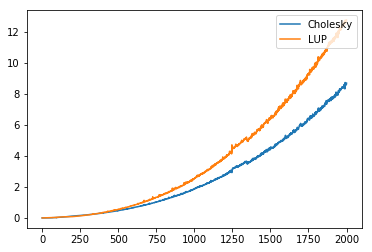
\includegraphics[width=0.8\linewidth]{execution_times_graph_N=2000.png}
    \caption{Comparaci\'on entre el tiempo de ejecuci\'on en segundos de los m\'etodos de factorización LUP y Cholesky para matrices de distintos tama\~nos.}
    \end{figure}

La  \textbf{Figura 2} representa la ejecuci\'on con el par\'metro $number=5$ para matrices generadas de tama\~no n x n, para $n \in \{5,10,15,...,2000\}$. Notemos que en este caso se ejecuto 5 veces cada factorizaci\'on y se calculo el promedio de los tiempos, obteniendo una curva m\'as suave (aunque tambi\'en se guardo la imagen en una diferente escala, por lo se ve m\'as n\'itida). \\

\textbf{Nota :} Para las gr\'aficas. Eje x: Tama\~no del lado la matriz. Eje y: Tiempo de ejecuci\'on en segundos.
    \begin{figure}[!h]
    \centering
    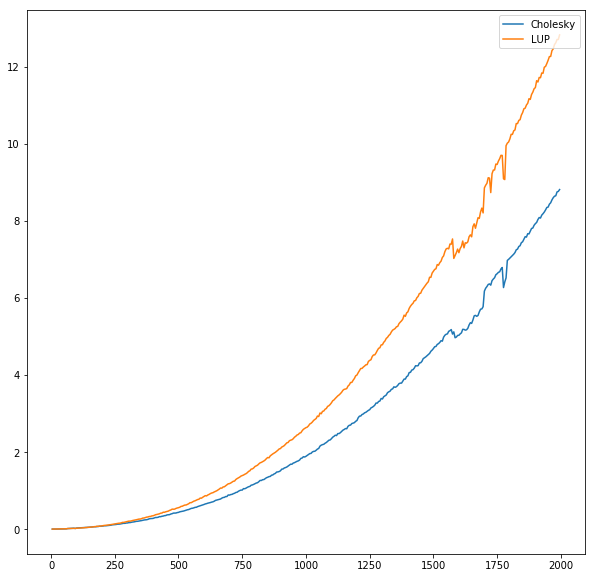
\includegraphics[width=0.8\linewidth,height=0.5\linewidth]{execution_times_graph_N=2000_smooth.png}
    \caption{Comparaci\'on entre el tiempo de ejecuci\'on en segundos de los m\'etodos de factorización LUP y Cholesky para matrices de distintos tama\~nos.}
    \end{figure}

\end{document}
